\documentclass{article}
\usepackage[T1]{fontenc}
\usepackage{lmodern}
\usepackage{graphicx}
\usepackage{amsmath,amssymb}
\usepackage[a4paper,margin=2cm]{geometry}
\usepackage[absolute,overlay]{textpos}
\setlength{\TPHorizModule}{1mm}
\setlength{\TPVertModule}{1mm}
\usepackage[indonesian]{babel}
\usepackage{hyperref}
\setlength{\emergencystretch}{2em}
% unit: Halaman 30

\begin{document}

% === Halaman 30 (llm) ===

\vspace{177.61mm}

Ada pertanyaan?

% deskripsi: Foto hitam putih sekelompok siswa di dalam kelas yang mengangkat tangan mereka untuk bertanya atau menjawab.
% bbox normalisasi: [0.1850, 0.2500, 0.7740, 0.8480]
\begin{textblock*}{123.69mm}(38.85mm,74.25mm)
\noindent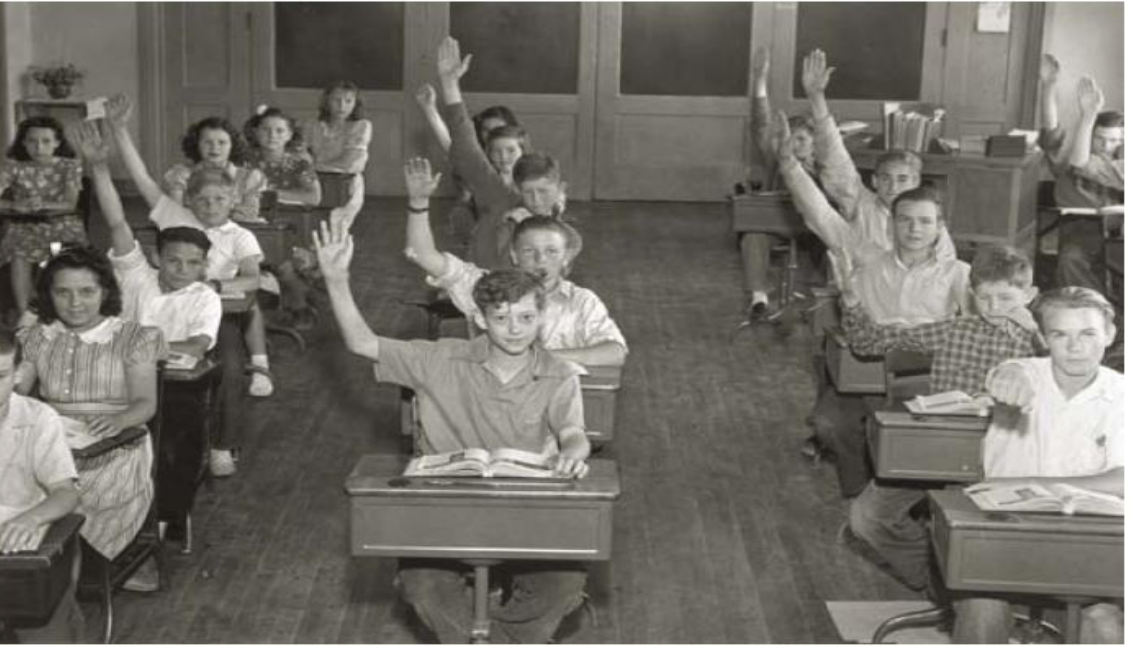
\includegraphics[width=123.69mm,height=177.61mm]{../../images/llm/page_030_img_01.png}%
\end{textblock*}

\end{document}
